\documentclass{lehramt-informatik-haupt}
\liLadePakete{mathe,formale-sprachen,tabelle}
\usepackage{tikz}
\usetikzlibrary{shapes.geometric,calc}

\begin{document}

\chapter{Formale Sprachen}

\section{Chomsky-Hierarchie\footcite{wiki:chomsky}}

Im Jahr 1957 veröffentlichte der amerikanische Sprachwissenschaftler
Noam \memph{Chomsky} ein Regelwerk, mit dessen Hilfe sich formale
Grammatiken in \memph{vier Klassen} einteilen lassen:
\footcite[Seite 168]{hoffmann}

\begin{description}
\item[Typ 0] Phrasenstrukturgrammatik

Jede Grammatik ist per Definition immer auch eine Typ-0-Grammatik.
Insbesondere unterliegt die Struktur der Produktionen \memph{keinen
weiteren vereinbarten Einschränkungen}.

\item[Typ 1] kontextsensitive Grammatik

Eine Grammatik heißt kontextsensitiv, wenn jede Produktionsregel $l
\rightarrow r$ entweder die Beziehung \memph{$|r| \geq |l|$} erfüllt
oder die Form \memph{$S \rightarrow \varepsilon$} aufweist. Ist die Regel
$S \rightarrow \varepsilon$ enthalten, so darf $S$ in keiner anderen
rechten Seite einer Regel vorkommen.

\item[Typ 2] kontextfreie Grammatik

Typ-2-Grammatiken sind dadurch charakterisiert, dass die \memph{linke
Seite} einer Produktionsregel ausschließlich aus einer \memph{einzigen
Variablen} besteht. Für alle Produktionen $l \rightarrow r$ gilt also $l
\in V$.

\item[Typ 3] reguläre Grammatik\footcite[Seite 14]{theo:fs:1}

Reguläre Grammatiken sind kontextfrei und besitzen die zusätzliche
Eigenschaft, dass die rechte Seite einer Produktion entweder aus dem
\memph{leeren Wort $\varepsilon$} oder einem \memph{Terminalsymbol},
\memph{gefolgt von einem Nonterminal}, besteht. Formal gesprochen
besitzt jede Produktion die Form $l \rightarrow r$ mit $l \in V$ und $r
\in \{ \varepsilon \} \cup \Sigma V$ .
\end{description}

\begin{center}
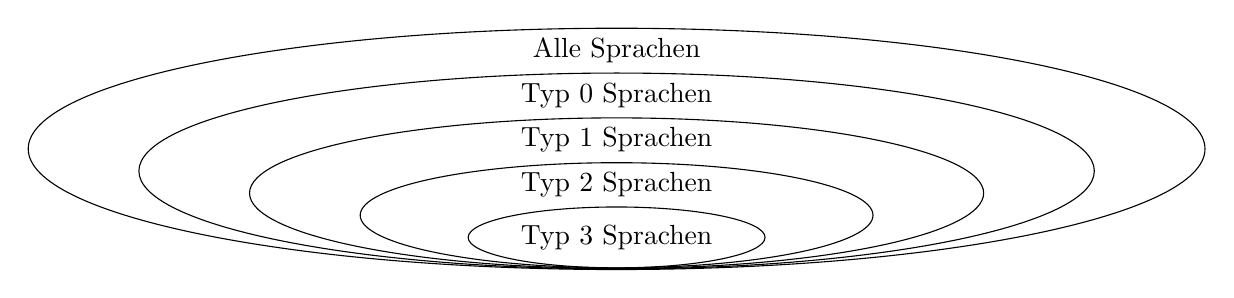
\begin{tikzpicture}[font=\rmfamily,breathe dist/.initial=0.01ex]
\foreach \X [count=\Y,remember=\Y as \LastY] in
{Typ 3 Sprachen, Typ 2 Sprachen, Typ 1 Sprachen, Typ 0 Sprachen, Alle Sprachen}
  {\ifnum\Y=1
  \node[ellipse,draw,outer sep=0pt] (F-\Y) {\X};
  \else
  \node[anchor=south] (T-\Y) at (F-\LastY.north) {\X};
  \path let \p1=($([yshift=\pgfkeysvalueof{/tikz/breathe dist}]T-\Y.north)-(F-\LastY.south)$),
  \p2=($(F-1.east)-(F-1.west)$),\p3=($(F-1.north)-(F-1.south)$)
  in ($([yshift=\pgfkeysvalueof{/tikz/breathe dist}]T-\Y.north)!0.5!(F-\LastY.south)$)
  node[minimum height=\y1,minimum width={\y1*\x2/\y3},
  draw,ellipse,inner sep=0pt] (F-\Y){};
  \fi}
\end{tikzpicture}
\end{center}

\noindent
Eine Sprache $L$ bezeichnen wir als Typ-$n$-Sprache, wenn eine
Typ-$n$-Grammatik $G$ existiert, die $L$ erzeugt. Die Menge aller
Typ-$n$-Sprachen notieren wir mit dem Symbol $\mathcal{L}_n$. Zwischen
den verschiedenen Sprachklassen besteht die folgende
Inklusionsbeziehung:

\begin{displaymath}
\mathcal{L}_0 \supset \mathcal{L}_1 \supset \mathcal{L}_2 \supset \mathcal{L}_3
\end{displaymath}

%-----------------------------------------------------------------------
%
%-----------------------------------------------------------------------

\section{Beispiel-Sprache je Sprach-Typ}

\begin{itemize}
\item \liAusdruck[L_3]{(ab)^n}{n \in \mathbb{N}}
ist regulär (Typ 3 Sprache)

\item \liAusdruck[L_2]{a^n b^n}{n \in \mathbb{N}}
ist kontextfrei (Typ 2 Sprache), aber nicht regulär

\item \liAusdruck[L_1]{a^n b^n c^n}{n \in \mathbb{N}}
ist kontextsensitiv (Typ 1 Sprache), aber nicht kontextfrei

\item \liAusdruck[L_0]{a^{(2^n)}}{n \in \mathbb{N}}
ist eine Typ 0 Sprache\footcite[Seite 15]{theo:fs:1}
\end{itemize}

%-----------------------------------------------------------------------
%
%-----------------------------------------------------------------------

Ein \memph{Terminalsymbol} (auch Terminalzeichen oder kurz Terminal
genannt) einer formalen Grammatik ist ein Symbol, das einzeln
\memph{nicht weiter durch eine Produktionsregel ersetzt werden
kann}.\footcite{wiki:terminal}

Eine Produktionsregel (auch Regel, Produktion oder Ersetzungsregel
genannt) ist in der Theorie formaler Grammatiken eine Regel, die angibt,
wie \memph{aus Wörtern durch eine Grammatik neue Wörter bzw.
Symbolfolgen produziert} werden.\footcite{wiki:produktionsregel}

%-----------------------------------------------------------------------
%
%-----------------------------------------------------------------------

\section{Abschlusseigenschaften}

In der Mathematik, insbesondere der Algebra, versteht man unter
Abgeschlossenheit einer Menge bezüglich einer Verknüpfung, dass die
Verknüpfung beliebiger Elemente dieser Menge wieder ein Element der
Menge ergibt. Beispielsweise ist die Menge der ganzen Zahlen
abgeschlossen bezüglich der Addition, Subtraktion und Multiplikation,
aber nicht bezüglich der Division.
\footcite{wiki:abgeschlossenheit}

\begin{description}

%%
%
%%

\item[$L_1 \cup L_2$ (Vereinigung):]

Die Vereinigung $L = L_1 \cup L_2$ zweier Sprachen $L_1$ und
$L_2$.\footcite{wiki:menge}

%%
%
%%

\item[$L_1 \cap L_2$ (Schnitt):]

Der Schnitt $L = L_1 \cap L_2$ zweier Sprachen $L_1$ und $L_2$.
\footcite{wiki:menge}

%%
%
%%

\item[$\bar L$ (Komplement):]

Das Komplement $\bar L = \Sigma^* \setminus L$ einer Sprache
$L$.
\footcite{wiki:komplement}

%%
%
%%

\item[$L_1 \circ L_2$ (Produkt / Konkatenation):]

Das Produkt \liAusdruck[]{uv}{u \in L_1 \lor v \in L_2} zweier
Sprachen $L_1$ und $L_2$.
\footcite{wiki:formale-sprache}

%%
%
%%

\item[$L^*$ (Kleene-Stern):]

Der Kleene-Stern $L^*$ einer Sprache $L$, \dh die beliebig
häufige Konkatenation von Wörter aus der Sprache $L$ vereinigt mit dem
leeren Wort.
\footcite[Seite 68]{theo:fs:1}
\footcite{wiki:kleensche-huelle}
\end{description}

{
\footnotesize
\begin{tabular}{r|c|c|c|c|c}
&
$L_1 \cup L_2$ &
$L_1 \cap L_2$  &
$\bar L$ &
$L_1 \circ L_2$ &
$L^*$ \\\hline
%     verein schnitt kompl produk kleene
Typ 3 & ja   & ja   & ja   & ja   & ja \\
Typ 2 & ja   & nein & nein & ja   & ja \\
Typ 1 & ja   & ja   & ja   & ja   & ja \\
Typ 0 & ja   & ja   & nein & ja   & ja \\
\end{tabular}
}
\footcite[Seite 33]{theo:fs:1}

%-----------------------------------------------------------------------
%
%-----------------------------------------------------------------------

\section{Entscheidbarkeitseigenschaften\footcite[Seite 591 Kapitel 19.1.3.3]{schneider}}

\begin{description}

%%
%
%%

\item[$\omega \in L(G)$ (Wortproblem):]

Als Wortproblem einer formalen Sprache bezeichnet man das
Entscheidungsproblem, zu einem \memph{gegebenen Wort} festzustellen, ob
dieses \memph{zur Sprache gehört}, oder nicht. Das Wortproblem einer
Sprache $L$ ist entscheidbar, wenn es einen Algorithmus gibt, der in
endlicher Zeit herausfindet, ob $\omega \in L(G)$ ist oder nicht.
\footcite{wiki:wortproblem}

%%
%
%%

\item[$L(G) = \emptyset$ (Leerheitsproblem):]

Als Leerheitsproblem bezeichnet man das Problem, zu entscheiden, ob eine
in Form einer formalen Grammatik gegebene \memph{formale Sprache $L$
leer ist}, also $L(G) = \emptyset$. Das Problem ist es also
herauszufinden, ob es Wörter gibt, die den Regeln der Grammatik genügen,
oder nicht.
\footcite{wiki:leerheitsproblem}

%%
%
%%

\item[$L(G_1) = L(G_2)$ (Äquivalenzproblem):]

Als Äquivalenzproblem bezeichnet man das Problem, zu entscheiden, ob
zwei formale Definitionen von zwei Sprachen $L_1$ und $L_2$
\memph{äquivalent} sind, also $L(G_1) = L(G_2)$ gilt.
\footcite[Seite 70-71]{theo:fs:1}
\footcite{wiki:aequivalenzproblem}

%%
%
%%

\item[$L(G_1) \cap L(G_2) = \emptyset$ (Schnittproblem):]

Als Schnittproblem bezeichnet man die Frage, ob die Schnittmenge zweier
formaler Sprachen, die durch Grammatiken gegeben sein sollen, leer ist.
\footcite{wiki:schnittproblem}

%%
%
%%

\item[$|L(G)| < \infty$ (Endlichkeitsproblem):]

Als Endlichkeitsproblem einer formalen Sprache $L$ bezeichnet man das
Problem, zu entscheiden, ob die Sprache endlich ist. Eine formale
Sprache wird als endlich bezeichnet, wenn die Menge ihrer
„Wörter“ endlich ist, man schreibt dann auch $|L| < \infty$.
\footcite{wiki:endlichkeitsproblem}
\end{description}

{
\footnotesize
\begin{tabular}{r|c|c|c|c|c}
&
$\omega \in L(G)$ &
$L(G) = \emptyset$ &
$L(G_1) = L(G_2)$ &
$L(G_1) \cap L(G_2) = \emptyset$ &
$|L(G)| < \infty$ \\\hline
%     wort   leer   äqui   schnitt end
Typ 3 & ja   & ja   & ja   & ja   & ja \\
Typ 2 & ja   & ja   & nein & nein & ja \\
Typ 1 & ja   & nein & nein & nein & nein \\
Typ 0 & nein & nein & nein & nein & nein \\
\end{tabular}
}

\section{Formale Sprachen und Maschinenmodelle\footcite[Seite 32]{theo:fs:3}}

\begin{tabular}{l|l|l}
Sprache & Maschinenmodell & Speichergröße \\\hline
Typ 3 & DFA, NFA & endlich\\
Typ 2 & DPDA, NPDA & Stapel\\
Typ 1 & LBA & proportional zu Eingabe\\
Typ 0 & DTM, NTM & unendlich\\
\end{tabular}

\noindent
\begin{tabularx}{\linewidth}{l|X||l|X}
Englisch & Bedeutung & Deutsch & Bedeutung \\\hline\hline

%%
%
%%

DFA\footcite{wiki:dfa} &
Deterministic Finite Automaton &
DEA &
Deterministischer Endlicher Automat\\

%%
%
%%

DPDA\footcite{wiki:dpda} &
Deterministic PushDown Automaton &
DKA &
Deterministischer Kellerautomat \\

%%
%
%%

TM, DTM\footcite{wiki:tm} &
Deterministic Turing machine &
&
Deterministische Turing-Maschine \\

%%
%
%%

LBA\footcite{wiki:lba} &
Linear Bounded Automaton &
&
Linear beschränkte Turingmaschine \\

%%
%
%%

NFA\footcite{wiki:nfa} &
Deterministic Finite Automaton &
NEA &
Nichtdeterministischer endlicher Automat\\

%%
%
%%

PDA, NPDA\footcite{wiki:pda} &
(Nondeterministic) PushDown Automaton &
KA, NKA &
Nichtdeterministischer Kellerautomat \\

%%
%
%%

NTM, NDTM\footcite{wiki:ntm} &
NonDeterministic Turing machine &
- &
Nichtdeterministische Turingmaschine\\
\end{tabularx}

\literatur

\end{document}
